\chapter{\ifproject%
\ifcpe การทดลองและผลลัพธ์\else Experimentation and Results\fi
\else%
\ifcpe การประเมินระบบ\else System Evaluation\fi
\fi}
บทนี้จะพูดถึงผลลัพธ์หลังจากที่ให้ทาง nursery ได้ลองใช้ web application ของเราและการแก้ไขตาม feedback ที่ได้รับ 
\section{Feedback จากทาง nursery หลังจากที่ได้ทดลองใช้ web application ครั้งแรก}
จากการที่ให้ user ได้ลองใช้งาน พบว่าเกือบทุก features นั้นสามารถใช้งานได้ตามความต้องการของทาง nursery แต่ยังมี features ที่ทาง nursery ทำการ feedback กลับมา โดยสรุปเป็นหัวข้อหลักๆ ได้ดังต่อไปนี้
\paragraph{ระบบบัญชี}
\begin{itemize}
    \item ยังไม่มีใบแจ้งยอดและใบเสร็จ
    \item ใบเสร็จไม่สามารถแนบสลิปจากภายนอกได้
    \item การเพิ่มรายการบัญชีไม่สามารถเลือกประเภทของสิ่งของต่างๆได้ 
\end{itemize}
\paragraph{ระบบคลังสินค้า}
\begin{itemize}
    \item ราคาของสินค้าไม่สามารถแก้ไขได้
    \item ไม่สามารถหักจำนวนของสินค้าอัตโนมัติได้
\end{itemize}

\section{การแก้ไขตาม feedback ที่ได้รับหลังจากการทดลองใช้งานครั้งแรก}
ใช้เวลาในการแก้ไขทั้งหมด 3 สัปดาห์ แล้วนำไปให้ทาง nursery ทดลองใช้อีกครั้ง โดยมีรายละเอียดการแก้ไขดังนี้
\paragraph{ระบบบัญชี}

\begin{figure}
  \begin{center}
    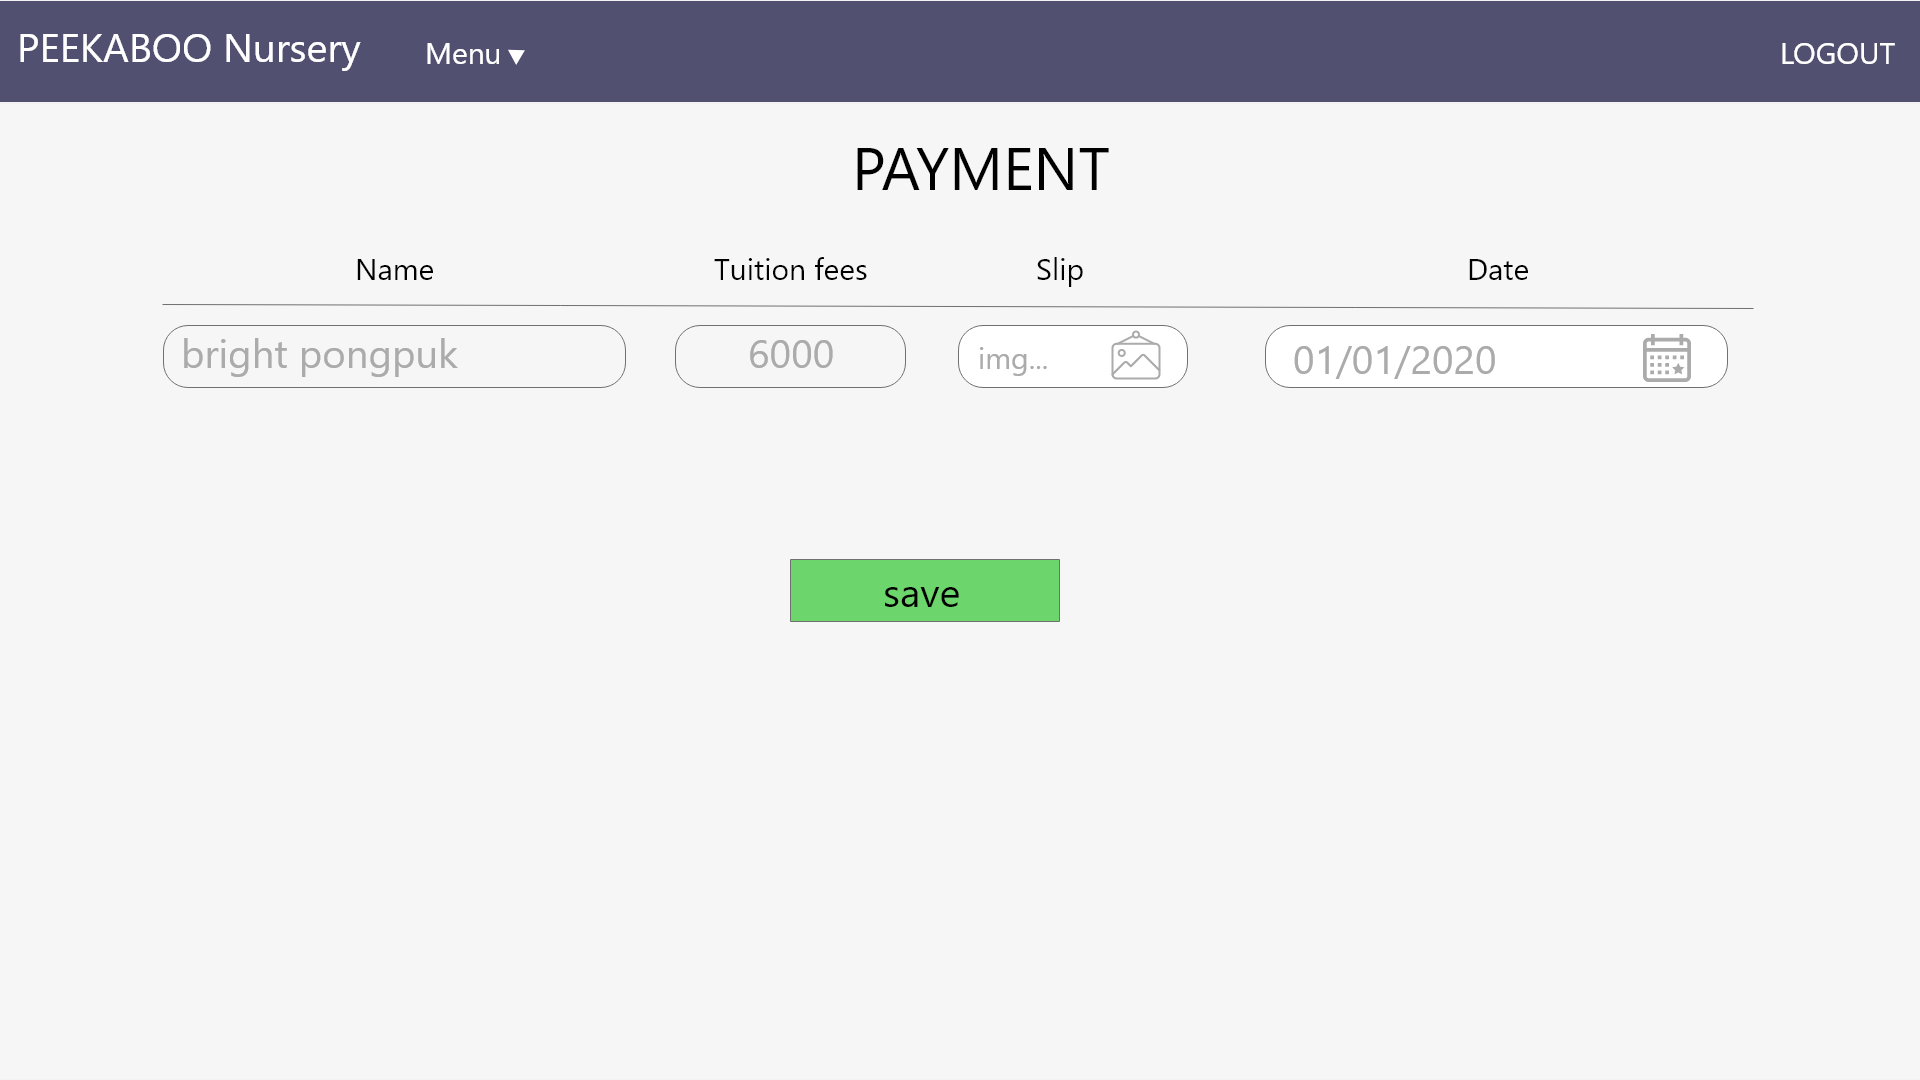
\includegraphics[width=\linewidth]{images/paymentPage.png}
  \end{center}
  \caption{หน้าระบบบัญชีเดิม}
  \label{fig:old1}
\end{figure}
\begin{itemize}
    \item เนื่องจากแบบเก่านั้น (รูปที่~\ref{fig:old1})   ไม่ได้แบ่งสีและเพิ่มสัญลักษณ์ ทำให้ผู้ใช้ยังสับสนอยู่ว่าถ้าต้องการทำแบบนี้จะต้องไปกดตรงไหน เราจึงแก้ให้สามารถเข้าใจได้ง่ายมากยิ่งขึ้น (รูปที่~\ref{fig:Payment})
    \item เพิ่มใบเสร็จและใบแจ้งยอด (รูปที่~\ref{fig:slipPage}, \ref{fig:invoicePage})
    \item ใบเสร็จสามารถแนบสลิปจากภายนอกได้ (รูปที่~\ref{fig:updatePayment})
    \item การเพิ่มรายการบัญชีสามารถเลือกประเภทของสิ่งของต่างๆ ได้ (รูปที่~\ref{fig:CreatePayment})
\end{itemize}

\paragraph{ระบบคลังสินค้า}
\begin{figure}
  \begin{center}
    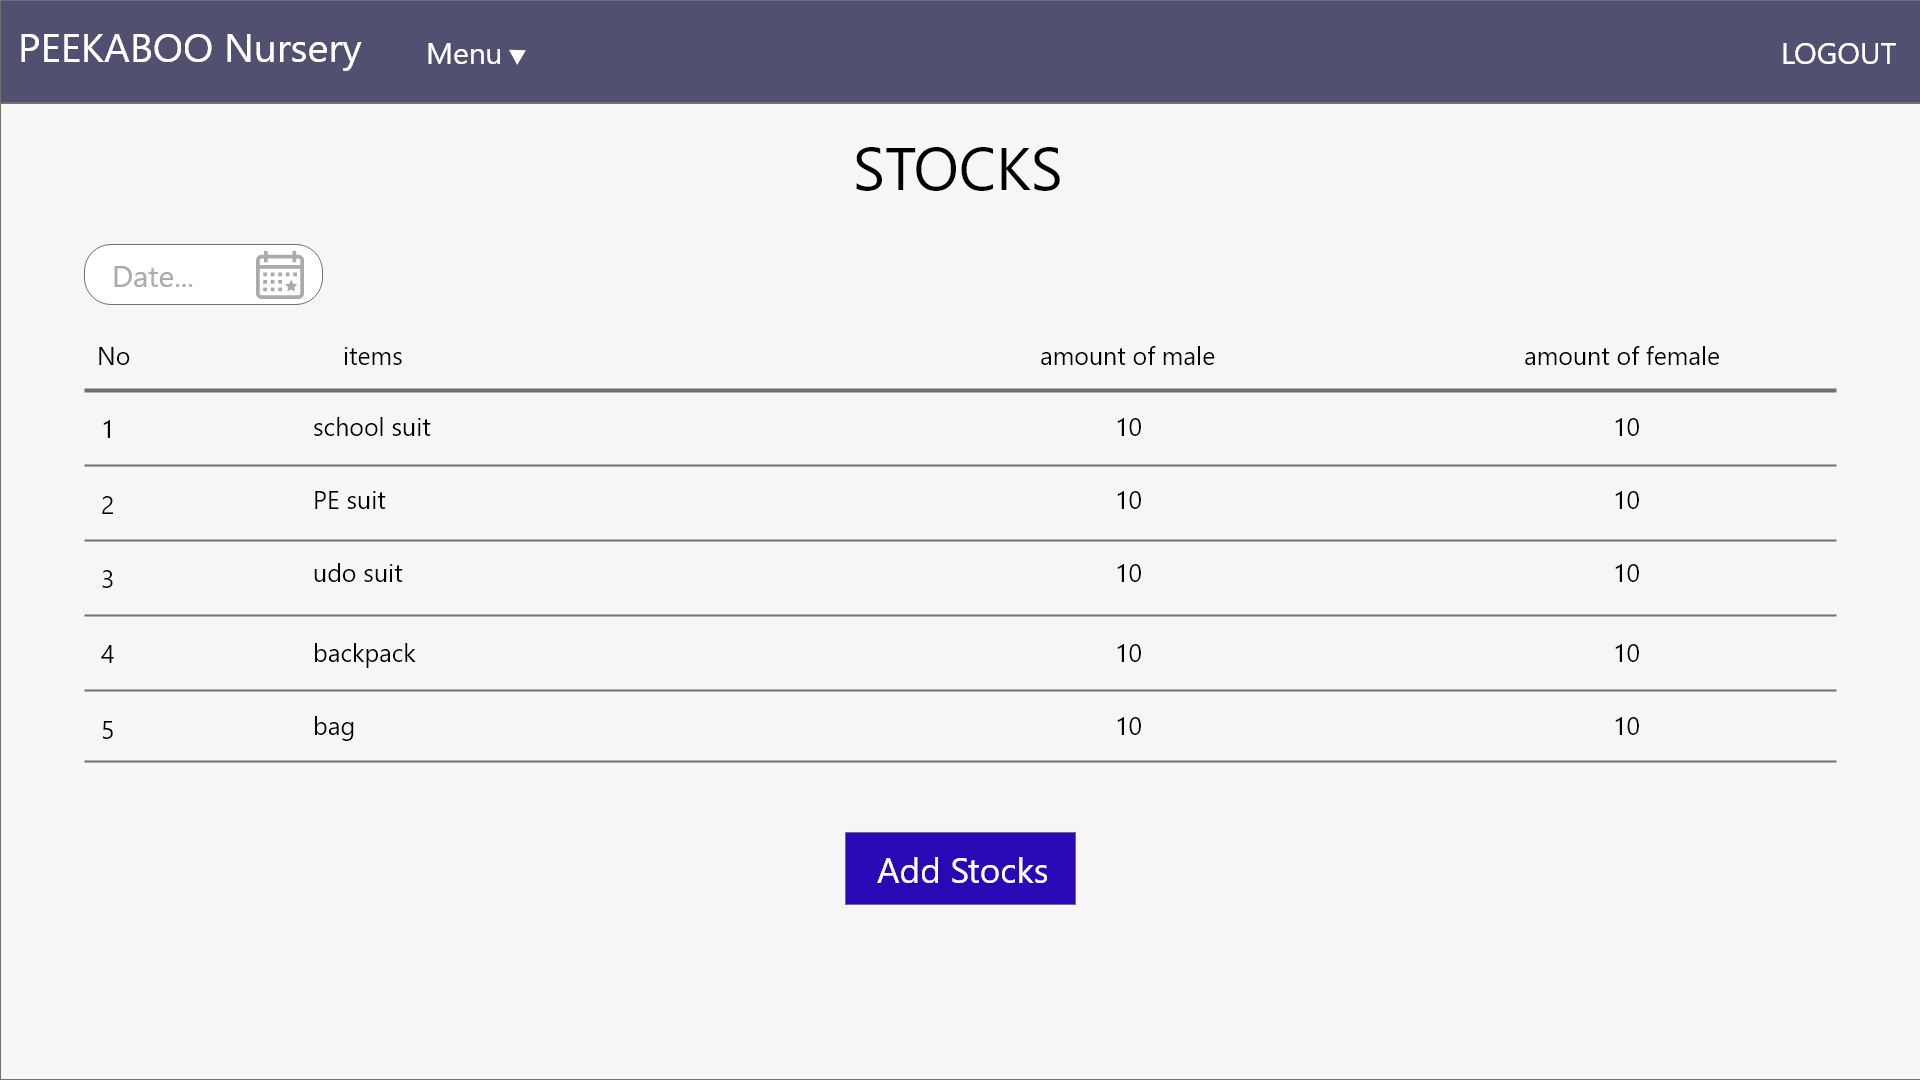
\includegraphics[width=\linewidth]{images/stockPage.png}
  \end{center}
  \caption{หน้าระบบคลังสินค้าเดิม}
  \label{fig:old2}
\end{figure}
\begin{itemize}
    \item เนื่องจากแบบเก่านั้น (รูปที่~\ref{fig:old2}) ยังไม่สามารถดู size ของสินค้าได้ ทำให้ผู้ใช้ไม่ทราบว่าสินค้า size นั้นๆ เหลือเท่าไหร่ ดังนั้น เราจึงแก้ไขให้สามารถดูจำนวนและ size ของสินค้านั้นๆ ได้ (รูปที่~\ref{fig:Stock})
    \item สามารถแก้ไขราคาของสินค้าได้ (รูปที่~\ref{fig:editPrice})
    \item สามารถหักจำนวนของสินค้าอัตโนมัติได้ (รูปที่~\ref{fig:CheckStock}, \ref{fig:HistoryStock})
\end{itemize}
\paragraph{หน้าประวัติ}
\begin{figure}
  \begin{center}
    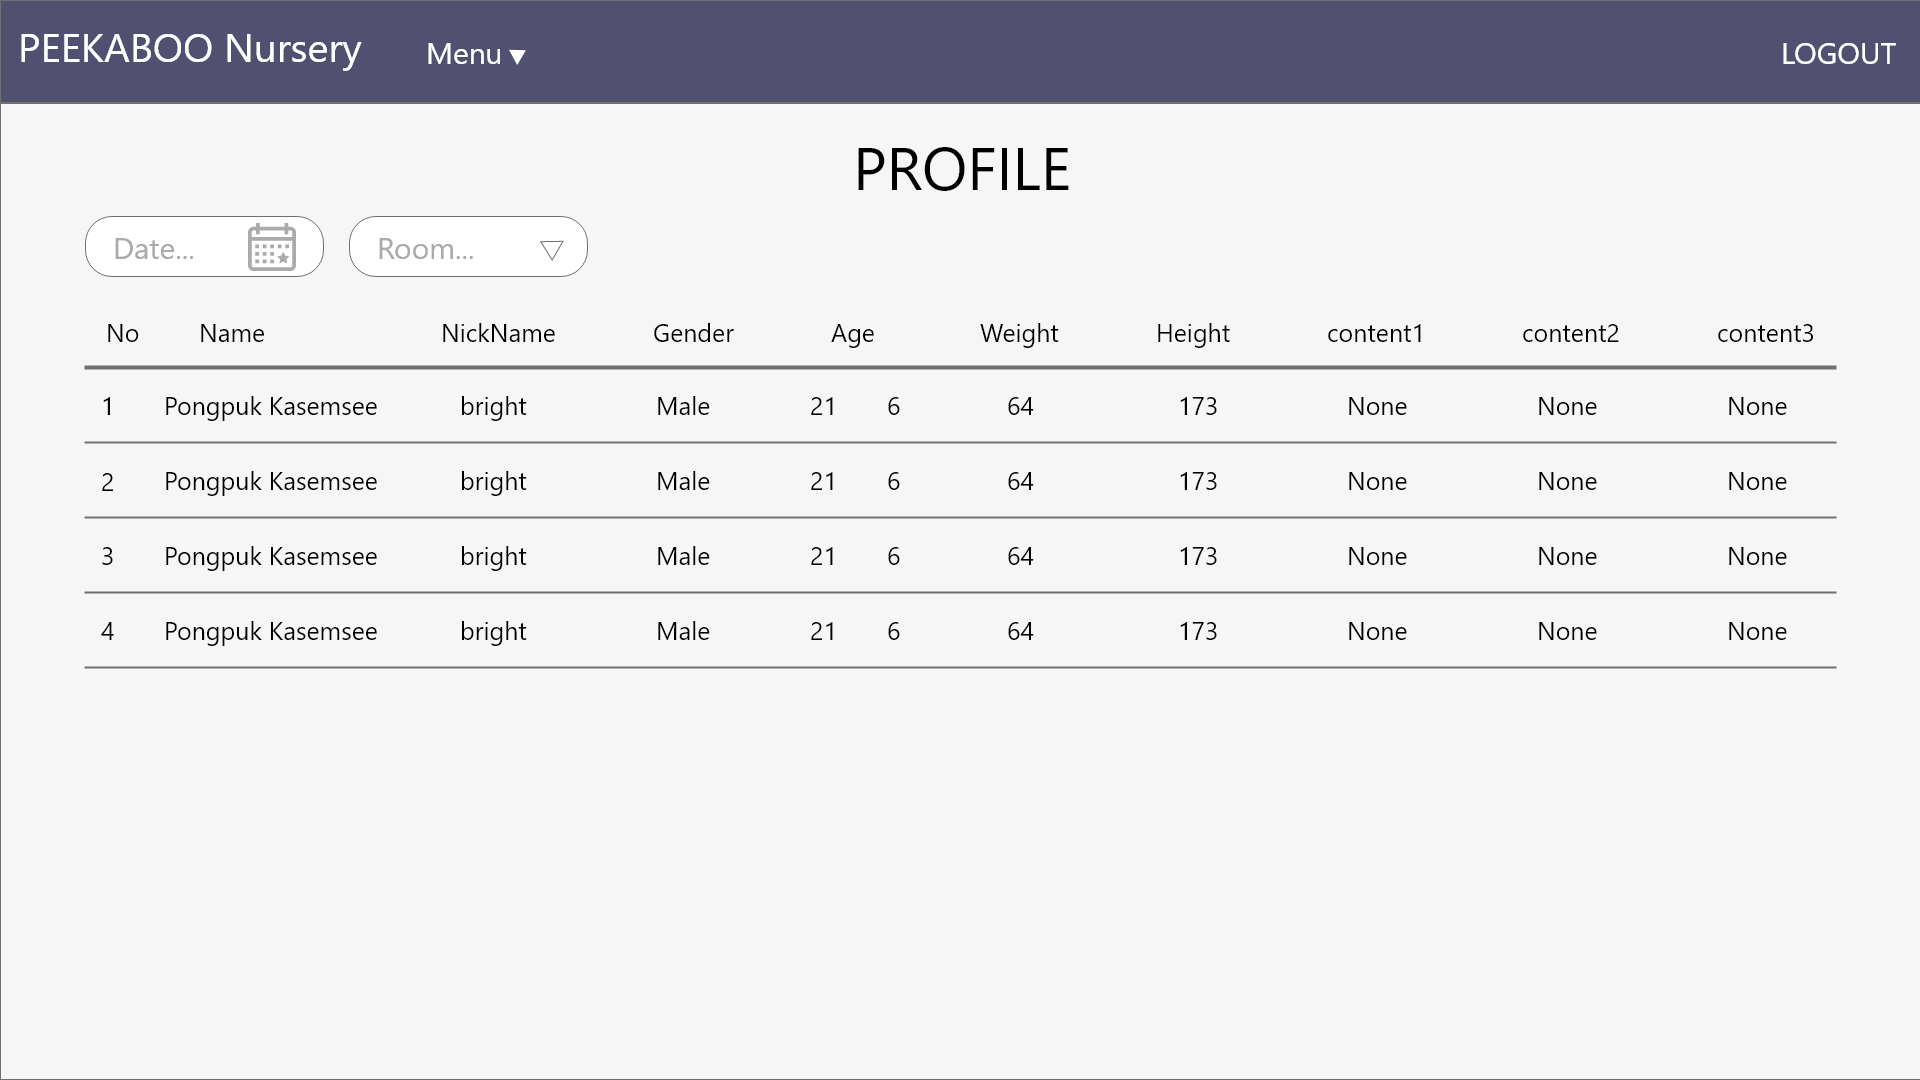
\includegraphics[width=\linewidth]{images/ProfileOnePage.png}
  \end{center}
  \caption{หน้าประวัติเดิม}
  \label{fig:old3}
\end{figure}
\begin{itemize}
    \item เนื่องจากแบบเก่านั้น (รูปที่~\ref{fig:old3}) ยังไม่มีสัญลักษณ์ สี และคำสั่งบางอย่าง ทำให้ผู้ใช้ยังติดขัดกับการทำงานอยู่ เราจึงแก้ไขให้ตรงตามความต้องการมากขึ้น (รูปที่~\ref{fig:Profile})
\end{itemize}



\section{ผลลัพธ์จากการประเมินหลังจากการแก้ไขตาม feedback}
ลำดับคะแนนจาก 1--5 นั้นนับจาก สามารถใช้งานยากที่สุด ไปยัง สามารถใช้งานง่ายที่สุด
\paragraph{ระบบลงทะเบียน}
\begin{itemize}
  \item จากการประเมินพบว่าสามารถใช้งานได้ง่าย และไม่พบปัญหาหลังจากทดลองใช้ (รูปที่~\ref{fig:Eval1})
\end{itemize}
\begin{figure}
  \begin{center}
    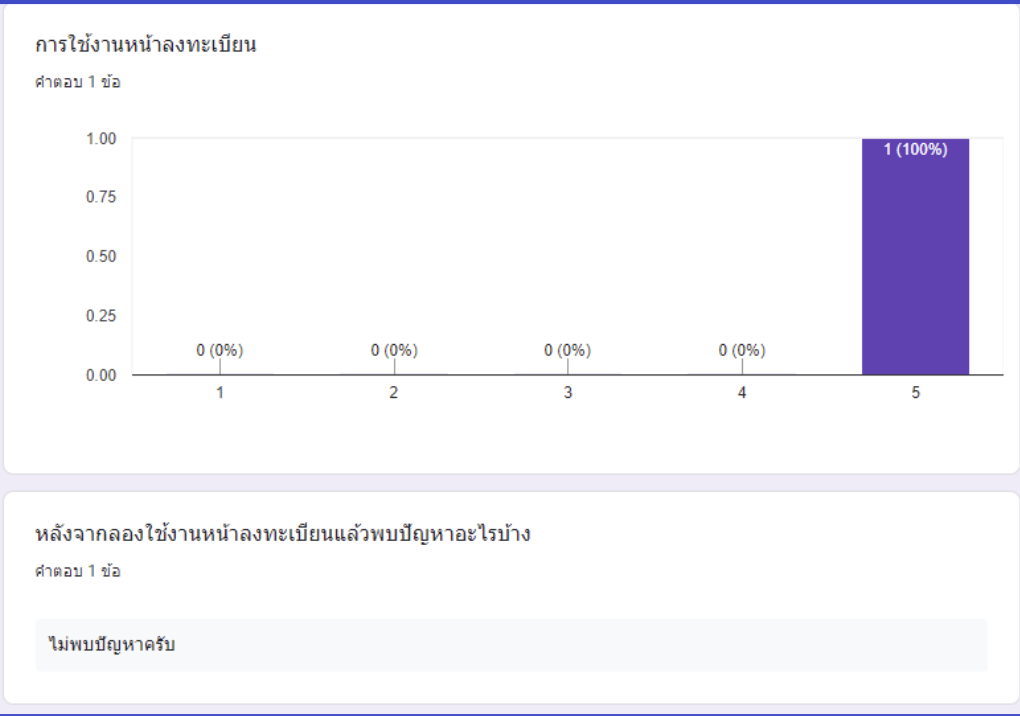
\includegraphics[width=\linewidth]{images/eval1.png}
  \end{center}
  \caption[ผลลัพธ์จากการประเมินการใช้งาน หน้าลงทะเบียน]{ผลลัพธ์จากการประเมินการใช้งาน หน้าลงทะเบียน}
  \label{fig:Eval1}
\end{figure}

\paragraph{หน้าประวัติ}
\begin{itemize}
  \item จากการประเมินพบว่าสามารถใช้งานได้ง่าย และไม่พบปัญหาหลังจากทดลองใช้ (รูปที่~\ref{fig:Eval2})
\end{itemize}
\begin{figure}
  \begin{center}
    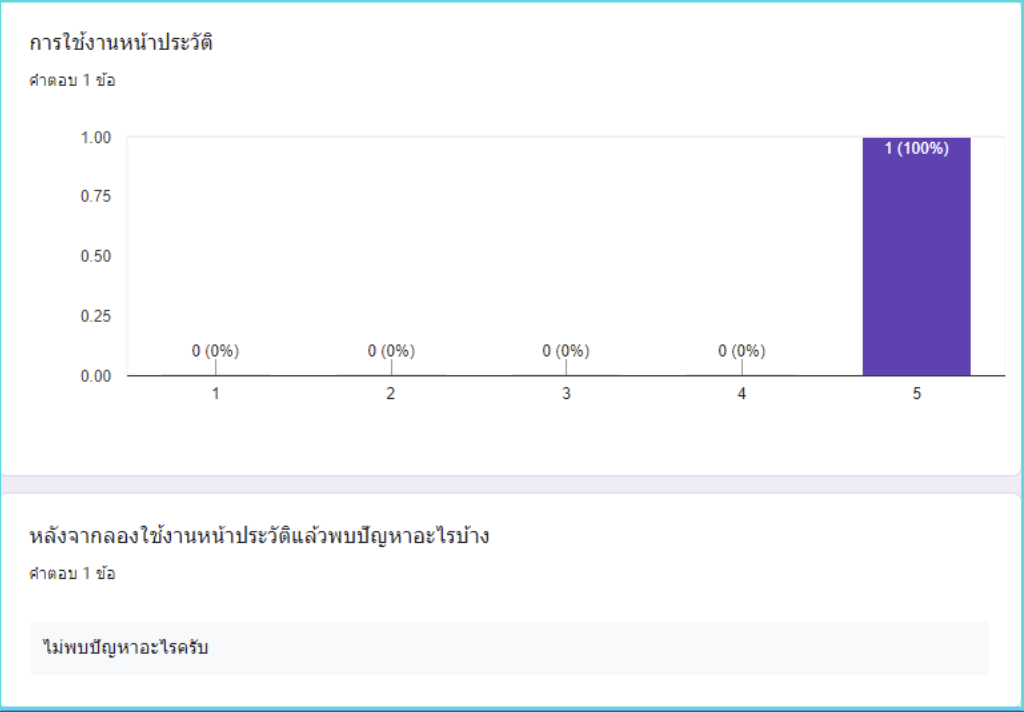
\includegraphics[width=\linewidth]{images/eval2.png}
  \end{center}
  \caption[ผลลัพธ์จากการประเมินการใช้งาน หน้าประวัติ]{ผลลัพธ์จากการประเมินการใช้งาน หน้าประวัติ}
  \label{fig:Eval2}
\end{figure}

\paragraph{ระบบเช็คชื่อรายวัน}
\begin{itemize}
  \item จากการประเมินพบว่าสามารถใช้งานได้ง่าย และไม่พบปัญหาหลังจากทดลองใช้ (รูปที่~\ref{fig:Eval3})
\end{itemize}
\begin{figure}
  \begin{center}
    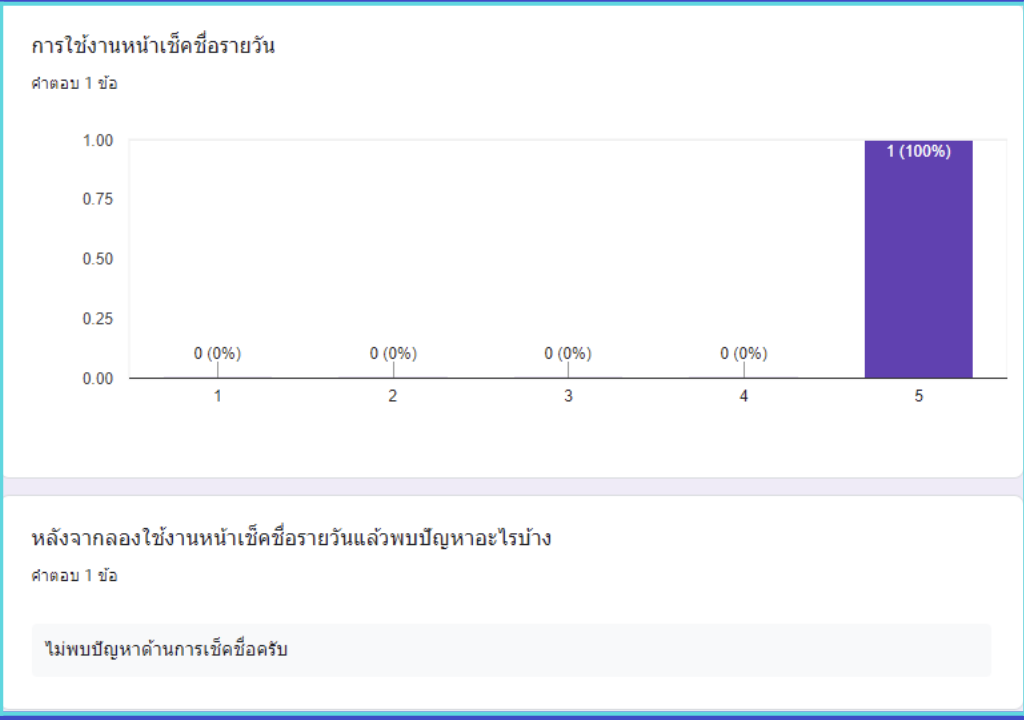
\includegraphics[width=\linewidth]{images/eval3.png}
  \end{center}
  \caption[ผลลัพธ์จากการประเมินการใช้งาน หน้าเช็คชื่อรายวัน]{ผลลัพธ์จากการประเมินการใช้งาน หน้าเช็คชื่อรายวัน}
  \label{fig:Eval3}
\end{figure}

\paragraph{ระบบเช็คสุขภาพรายวัน}
\begin{itemize}
  \item จากการประเมินพบว่าสามารถใช้งานได้ง่าย และไม่พบปัญหาหลังจากทดลองใช้ (รูปที่~\ref{fig:Eval5})
\end{itemize}
\begin{figure}
  \begin{center}
    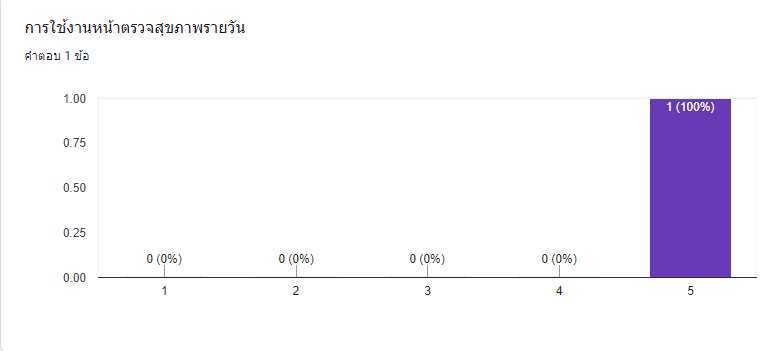
\includegraphics[width=\linewidth]{images/eval5.png}
  \end{center}
  \caption[ผลลัพธ์จากการประเมินการใช้งาน ตรวจสุขภาพรายวัน]{ผลลัพธ์จากการประเมินการใช้งาน ตรวจสุขภาพรายวัน}
  \label{fig:Eval5}
\end{figure}

\paragraph{ระบบเช็คอุปกรณ์รายวัน}
\begin{itemize}
  \item จากการประเมินพบว่าสามารถใช้งานได้ง่าย และไม่พบปัญหาหลังจากทดลองใช้ (รูปที่~\ref{fig:Eval6})
\end{itemize}
\begin{figure}
  \begin{center}
    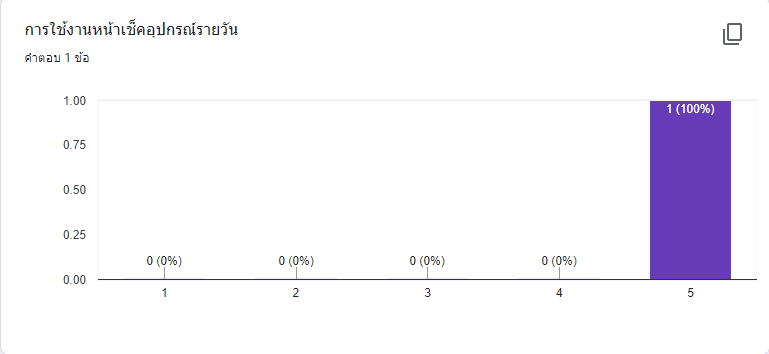
\includegraphics[width=\linewidth]{images/eval6.png}
  \end{center}
  \caption[ผลลัพธ์จากการประเมินการใช้งาน เช็คอุปกรณ์รายวัน]{ผลลัพธ์จากการประเมินการใช้งาน เช็คอุปกรณ์รายวัน}
  \label{fig:Eval6}
\end{figure}

\paragraph{ระบบบัญชี}
\begin{itemize}
  \item จากการประเมินพบว่าสามารถใช้งานได้ง่าย และไม่พบปัญหาหลังจากทดลองใช้ (รูปที่~\ref{fig:Eval7})
\end{itemize}
\begin{figure}
  \begin{center}
    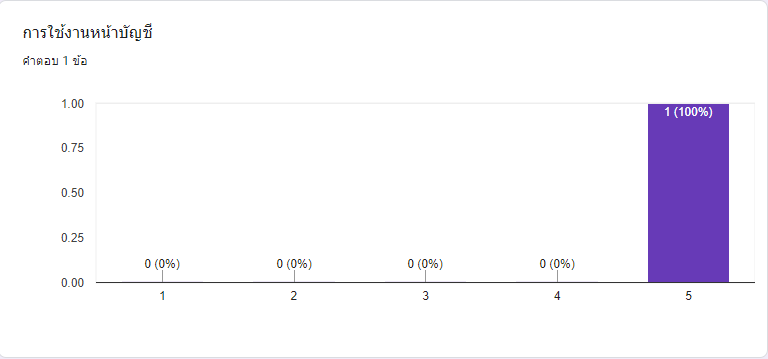
\includegraphics[width=\linewidth]{images/eval7.png}
  \end{center}
  \caption[ผลลัพธ์จากการประเมินการใช้งาน ระบบบัญชี]{ผลลัพธ์จากการประเมินการใช้งาน ระบบบัญชี}
  \label{fig:Eval7}
\end{figure}

\paragraph{ระบบคลังสินค้า}
\begin{itemize}
  \item จากการประเมินพบว่าสามารถใช้งานได้ง่าย และไม่พบปัญหาหลังจากทดลองใช้ (รูปที่~\ref{fig:Eval8})
\end{itemize}
\begin{figure}
  \begin{center}
    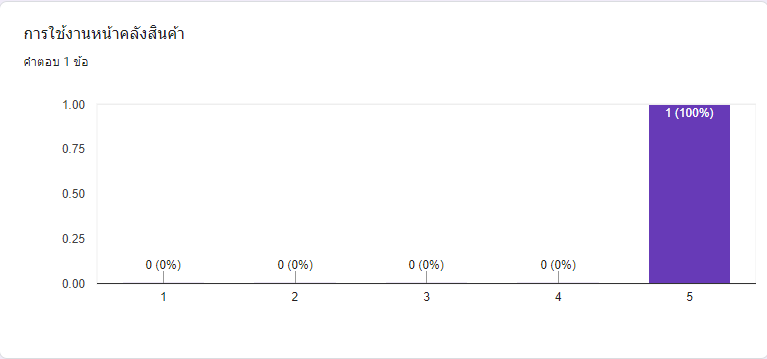
\includegraphics[width=\linewidth]{images/eval8.png}
  \end{center}
  \caption[ผลลัพธ์จากการประเมินการใช้งาน ระบบคลังสินค้า]{ผลลัพธ์จากการประเมินการใช้งาน ระบบคลังสินค้า}
  \label{fig:Eval8}
\end{figure}


\paragraph{สรุปผลการประเมินของระบบต่างๆ}
\begin{itemize}
  \item ทุก features ที่เราแก้ไขนั้นสามารถใช้งานได้ง่ายและสะดวกต่อทาง nursery มากยิ่งขึ้นและไม่พบปัญหาจากการใช้งานในแต่ละ feature (รูปที่~\ref{fig:Eval4})
\end{itemize}
\begin{figure}
  \begin{center}
    
\includegraphics[width=\linewidth]{images/eval4.png}
  \end{center}
  \caption[Comments จากผู้ใช้งาน]{Comments จากผู้ใช้งาน}
  \label{fig:Eval4}
\end{figure}

